

\begin{tabularx}{\textwidth}{| X | X | X |}
    \hline \textbf{Elemento} & \textbf{Descripción} & \textbf{Importancia} \\
    \hline \textbf{Datos básicos} & Usuarios: Jugadores de \gls{gbfvs} \newline Limitaciones: No se puede comparar todas las movidas de un personaje con todas de otro  & Si un usuario no es jugador de \gls{gbfvs}, no le va a conseguir utilidad a la aplicación\\
    \hline \textbf{Características físicas} & La audiencia para la aplicación es aquellos de 13 años o mas, independiente de genero o sexo. Si el usuario puede navegar el internet, puede acceder la aplicación & \gls{gbfvs}, como muchos juegos de pelea, son bien accesibles a personas con discapacidades. Es por esto, se piensa seguir las guías de accesibilidad para la \textit{web}\\ 
    \hline \textbf{Características psicológicas} & Se asume que el usuario es alfabeta, conoce la notación de teclado numérico \cite{noauthor_numpad_nodate} y conoce acerca de \gls{frame_data} & Debido a la manera que se extrae la data de su fuente de origen, el usuario debe ser capaz de comprender la notación de teclado numérico\\
    \hline \textbf{Dispositivos comúnmente usados} & La aplicación es una página \textit{web}, por ende, cualquier dispositivo que pueda navegar el internet, puede acceder la aplicación.  & La mayoría de la demografía de la aplicación tienen acceso a un dispositivo móvil a todo momento. \\
\end{tabularx}

\begin{tabularx}{\textwidth}{| X |  X |  X |}
    & Sin embargo, la aplicación está diseñada principalmente para dispositivos móviles y computadoras & Este punto es importante porque la aplicación es útil cuando se esté compitiendo\\
    \hline \textbf{Modelo mental del sistema} &  & \\ 
    \hline \textbf{Metas} & Al iniciar, se le ofrece al usuario las entradas de el el personaje que inició el ataque, el que respondió al ataque y sus respectivas movidas de cada personaje seleccionado. Al llegar a la página de resultados, el usuario logro seleccionar el personaje que inició el ataque, el que respondió al ataque y sus respectivas movidas y logró ver como son los datos fotográmicos de las movidas al ser comparadas & Dado que la naturaleza de la aplicación es de calculadora fotográmica, es obvio entonces que es de gran importancia que el usuario consiga la información que busca \\ 
    \hline \textbf{Requisitos} & Se piensa que la aplicación sera utilizada espontáneamente entre o antes partidas. Es por esto que aplicación debe ser sencilla y rápida de acceder & La rapidez y sencillez y sumamente importante debido a que el tiempo entre partidas en un torneo es bien corto (entre 1-3 minutos). Se tiene que tener acceso inmediato a la información deseada\\ 
    \hline
\end{tabularx}

\textbf{Metáfora de la interfaz gráfica}: Los juegos de pelea generalmente tienen un diseño de similar a dos cajas verticales, como se puede apreciar en la figura \ref{fig: abstract model}:

\begin{figure}[ht!]
    \centering
    \caption{Modelo abstracto del menú de los juegos de pelea}
    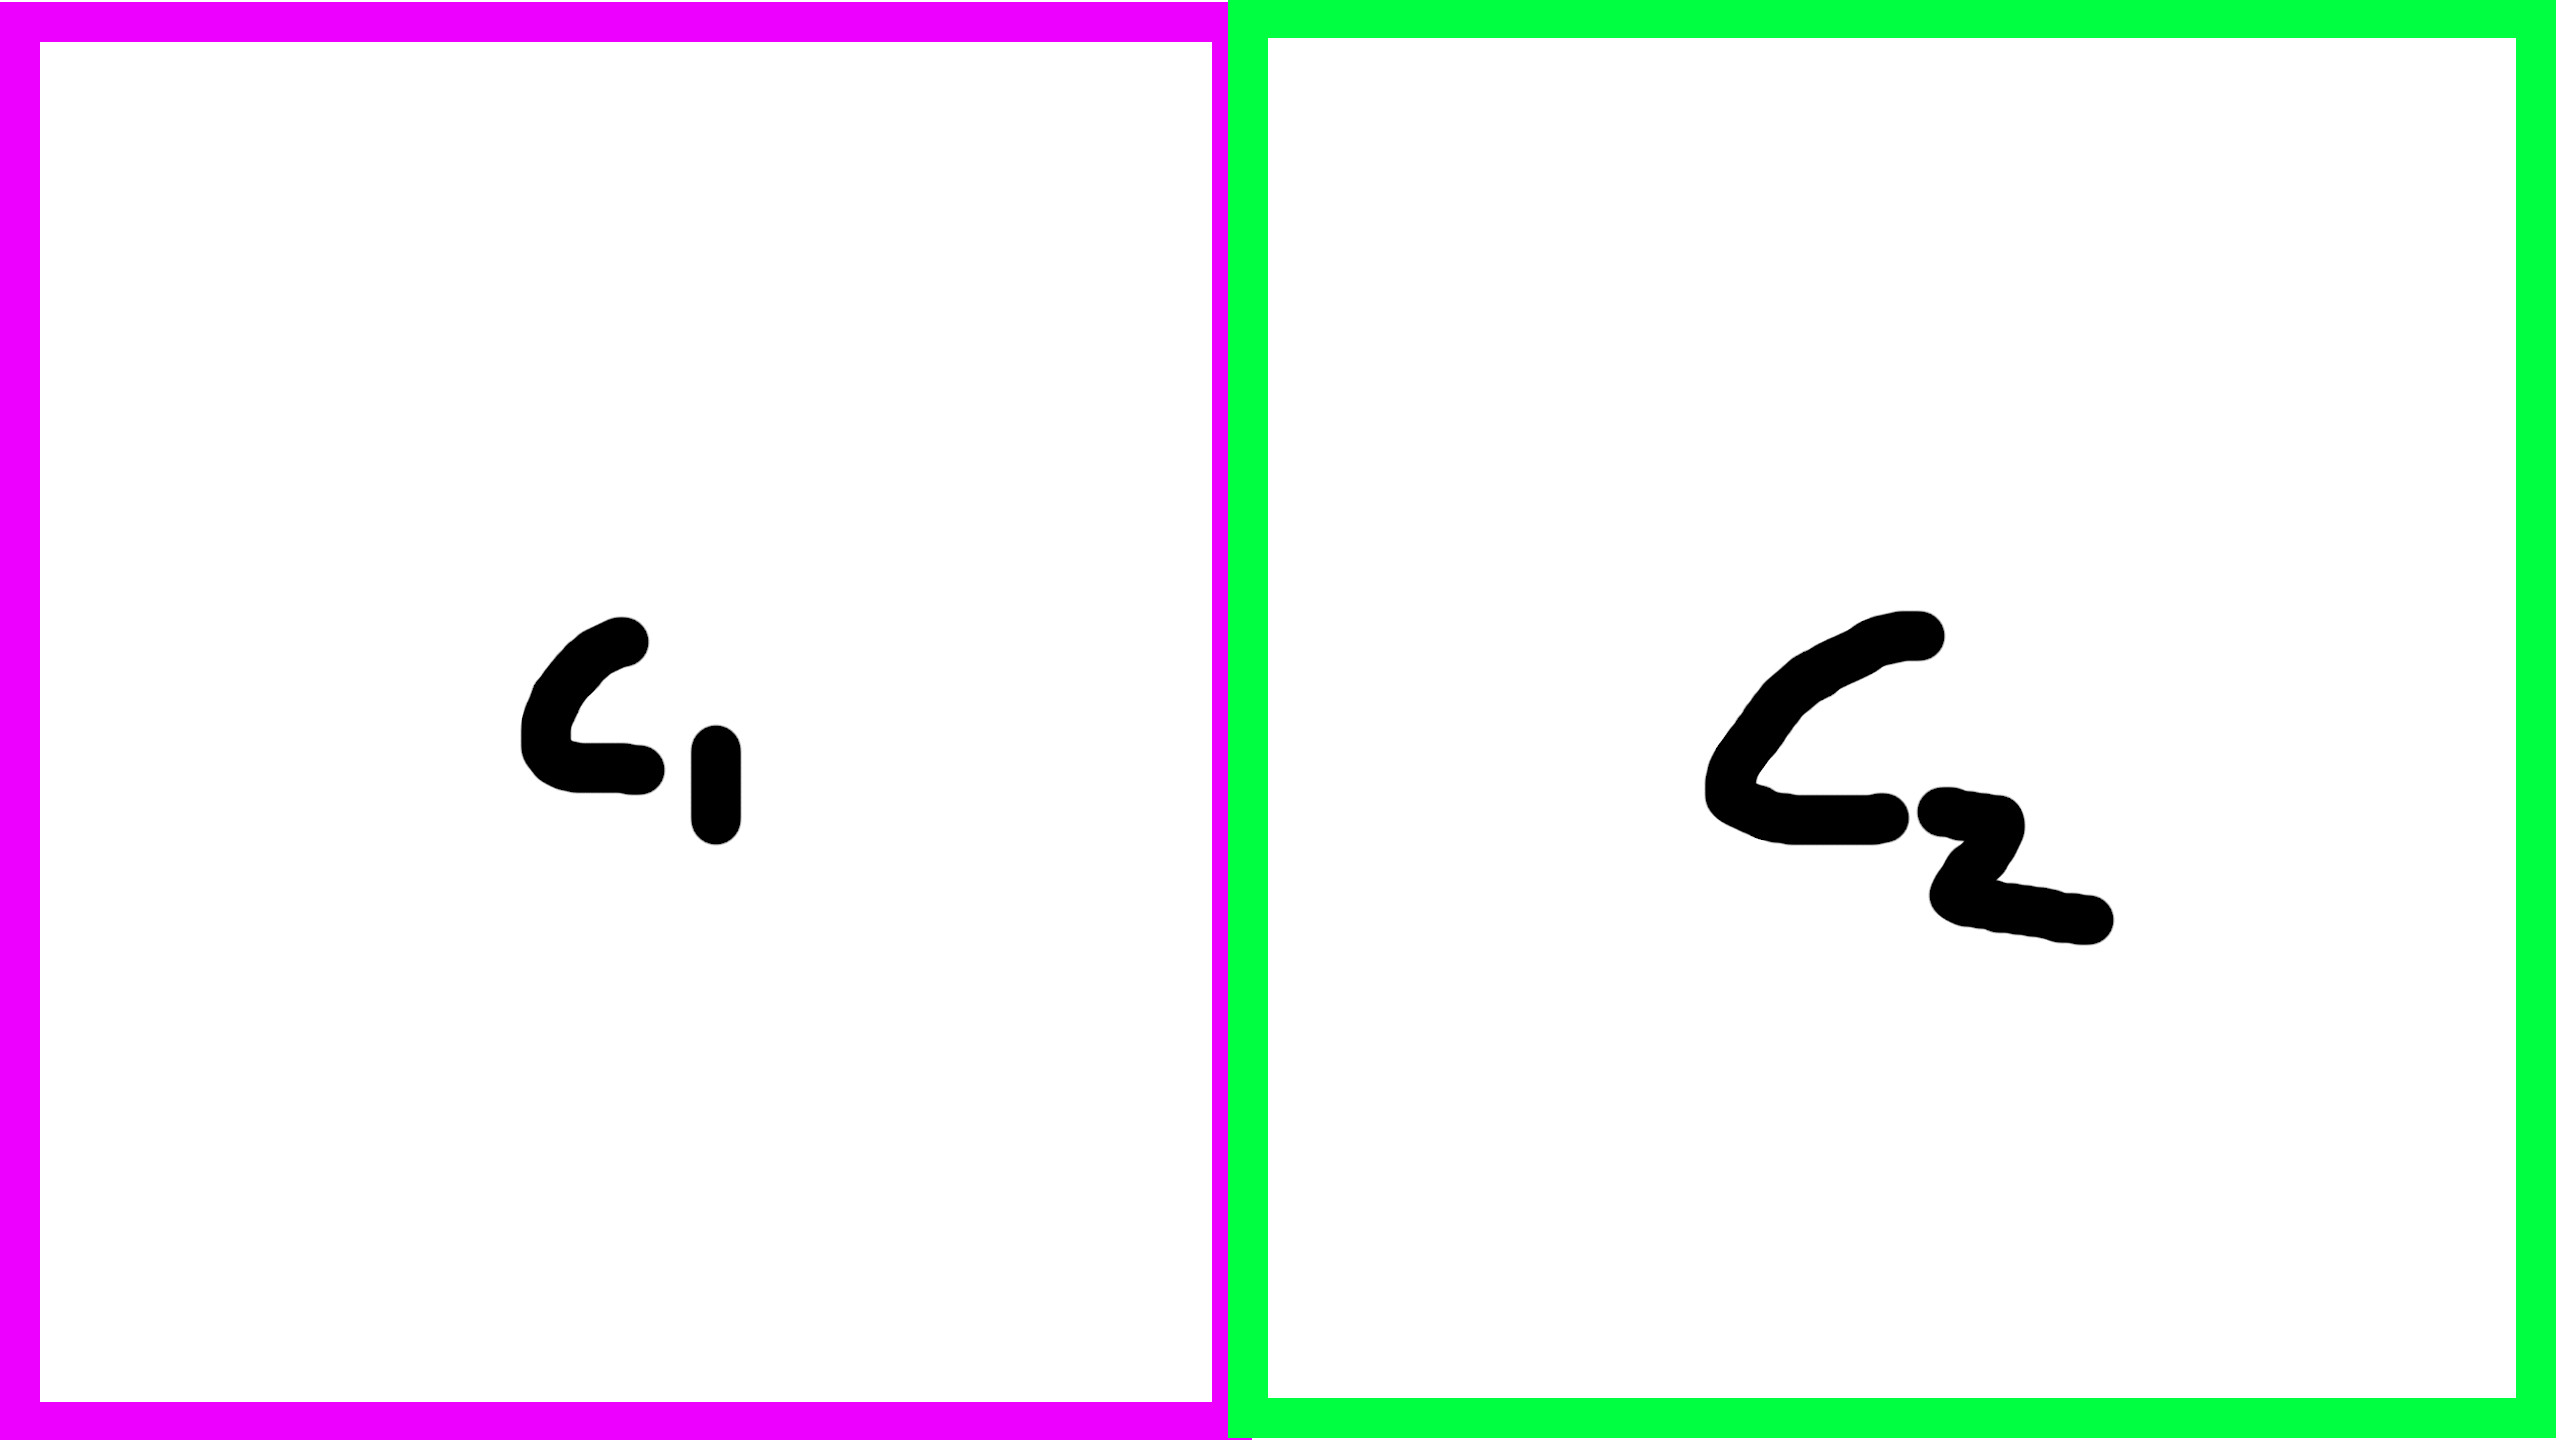
\includegraphics[height=0.2\textwidth]{figures/abstract-design.jpg}
    \label{fig: abstract model}
\end{figure}

Dentro de estas dos cajas, están los personajes que se han seleccionado y su color de traje, como se puede ver en la figura \ref{fig: strive chracter select}:

\begin{figure}[ht!]
    \centering
    \caption{Menú de selección de personaje de Guilty Gear Strive}
    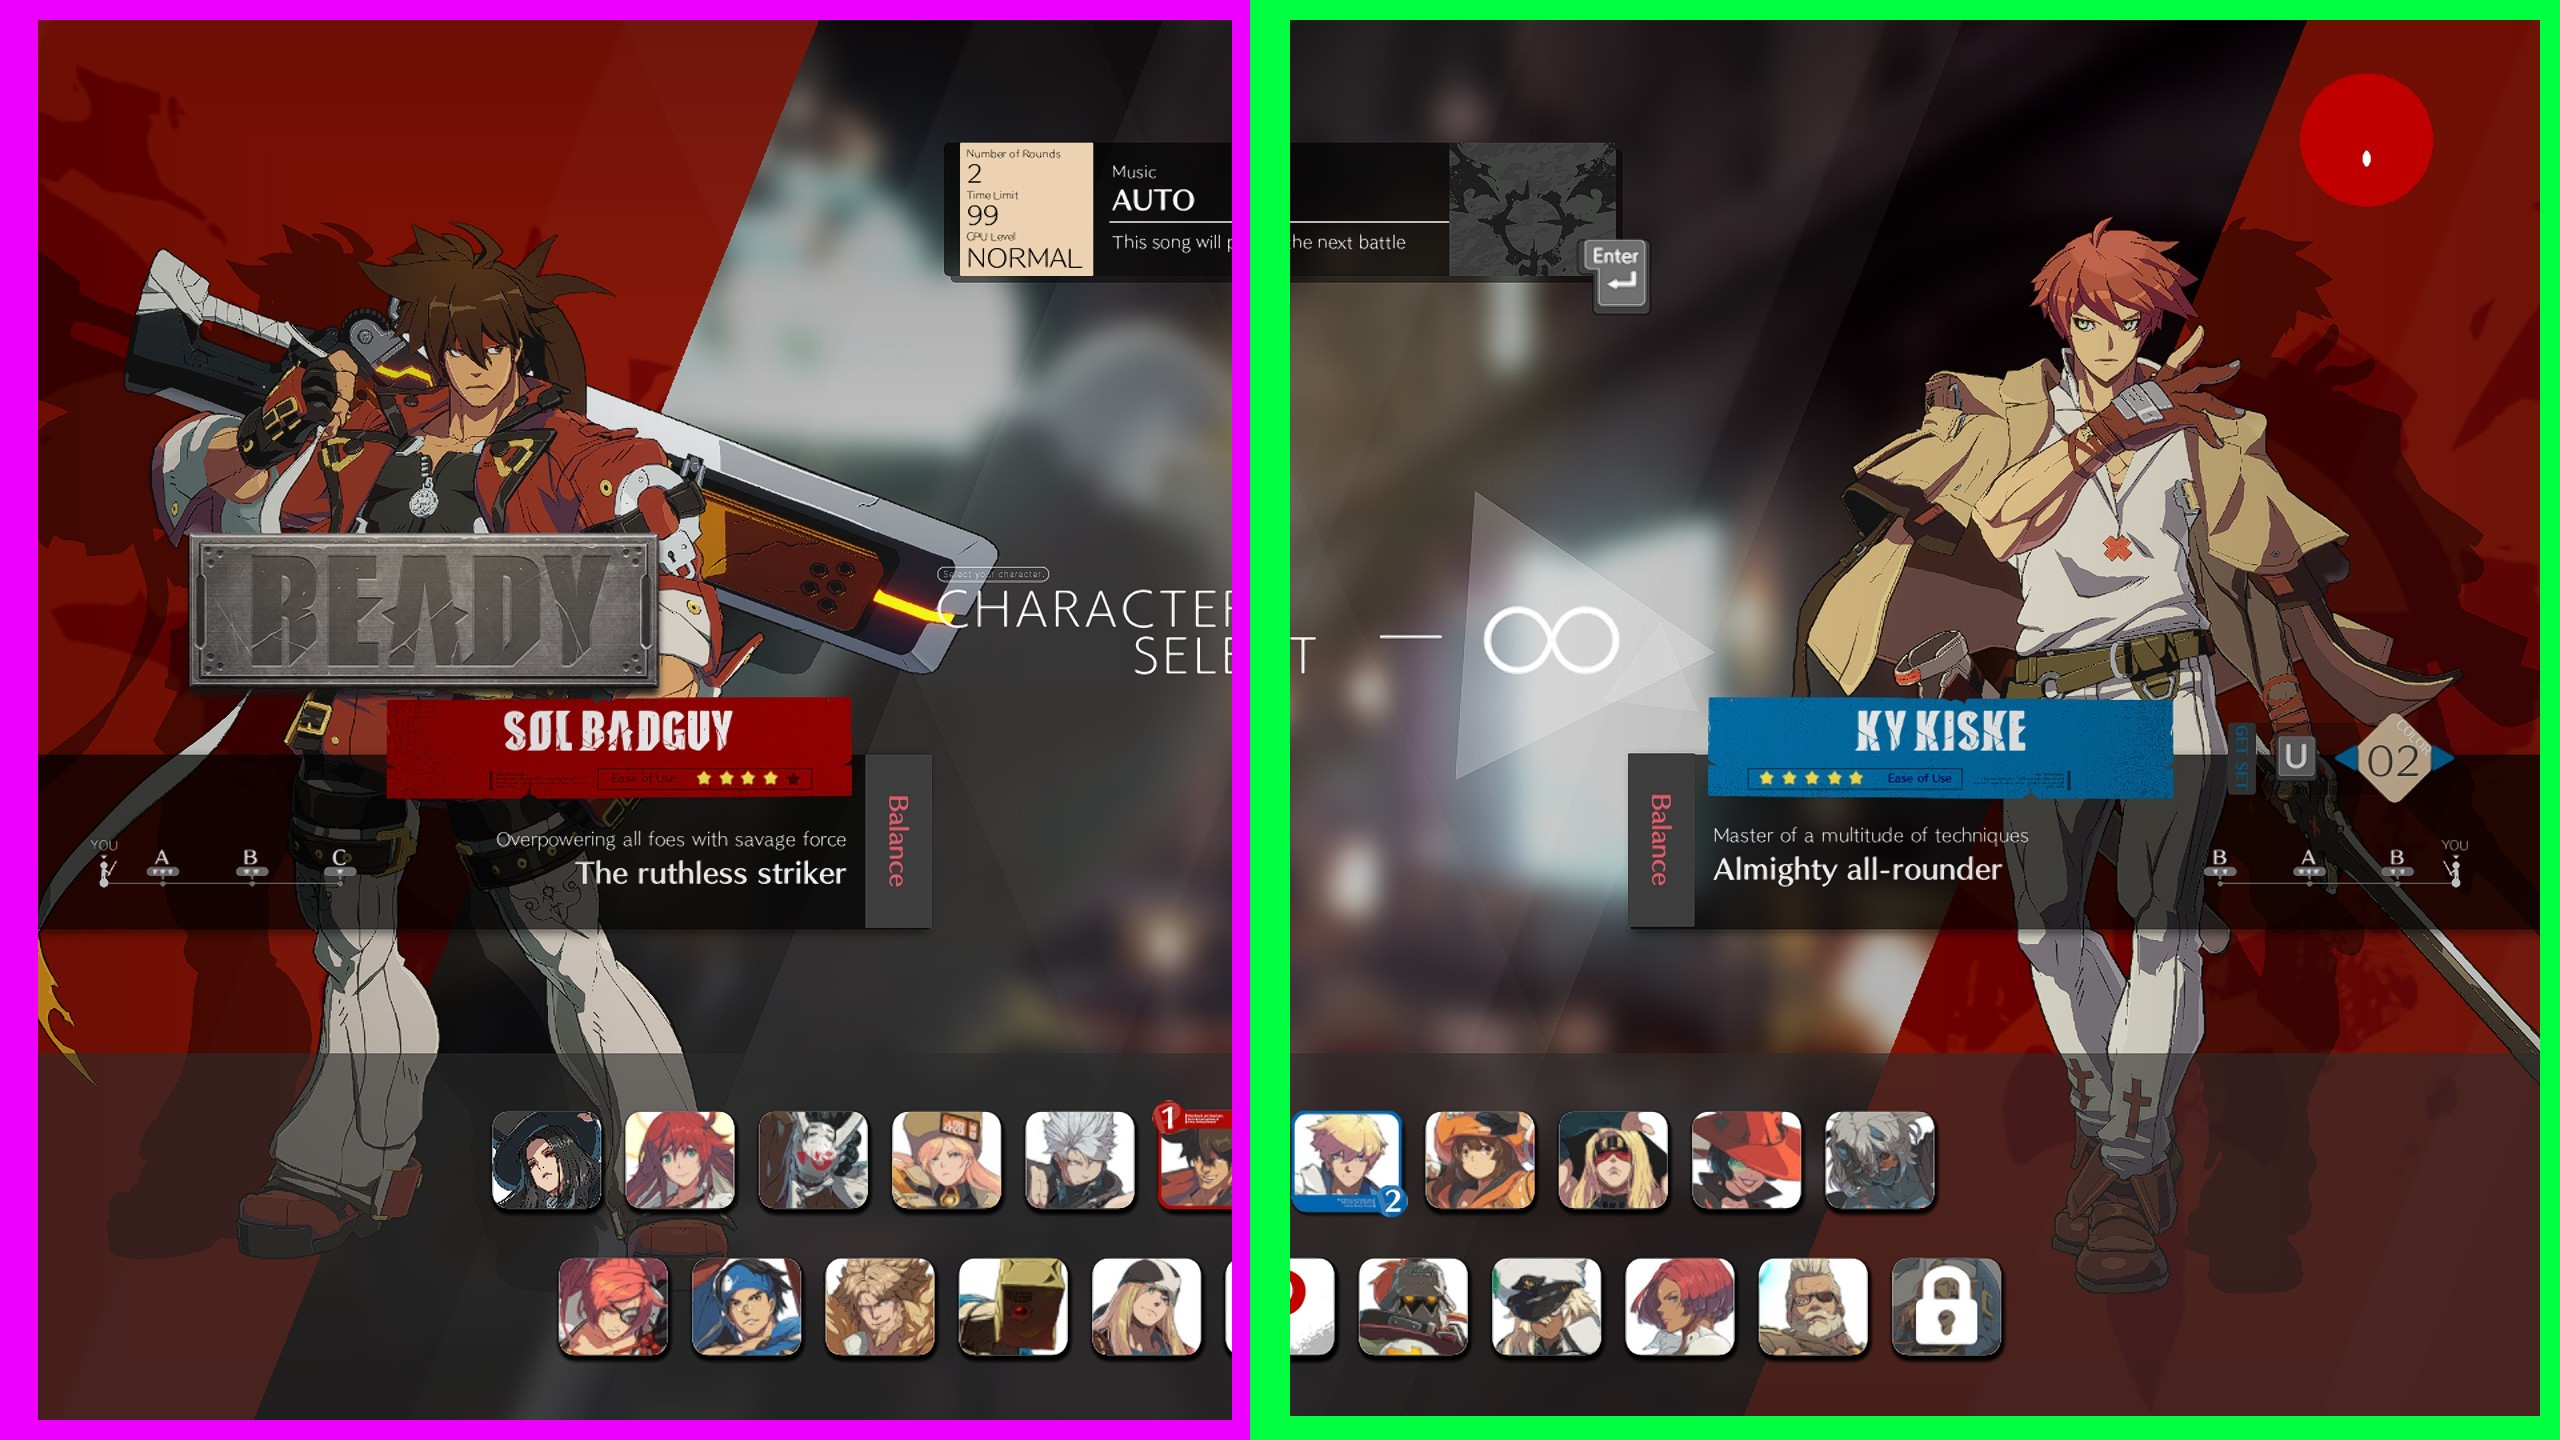
\includegraphics[height=0.5\textwidth]{figures/guilty.jpg}
    \label{fig: strive chracter select}
\end{figure}

Lo mismo ocurre en otros juegos como Melty Blood: Type Lumina \cite{noauthor_melty_nodate}, la figura \ref{fig: melty character select}:

\begin{figure*}[ht!]
    \centering
    \caption{Menú de selección de personaje de Melty Blood}
    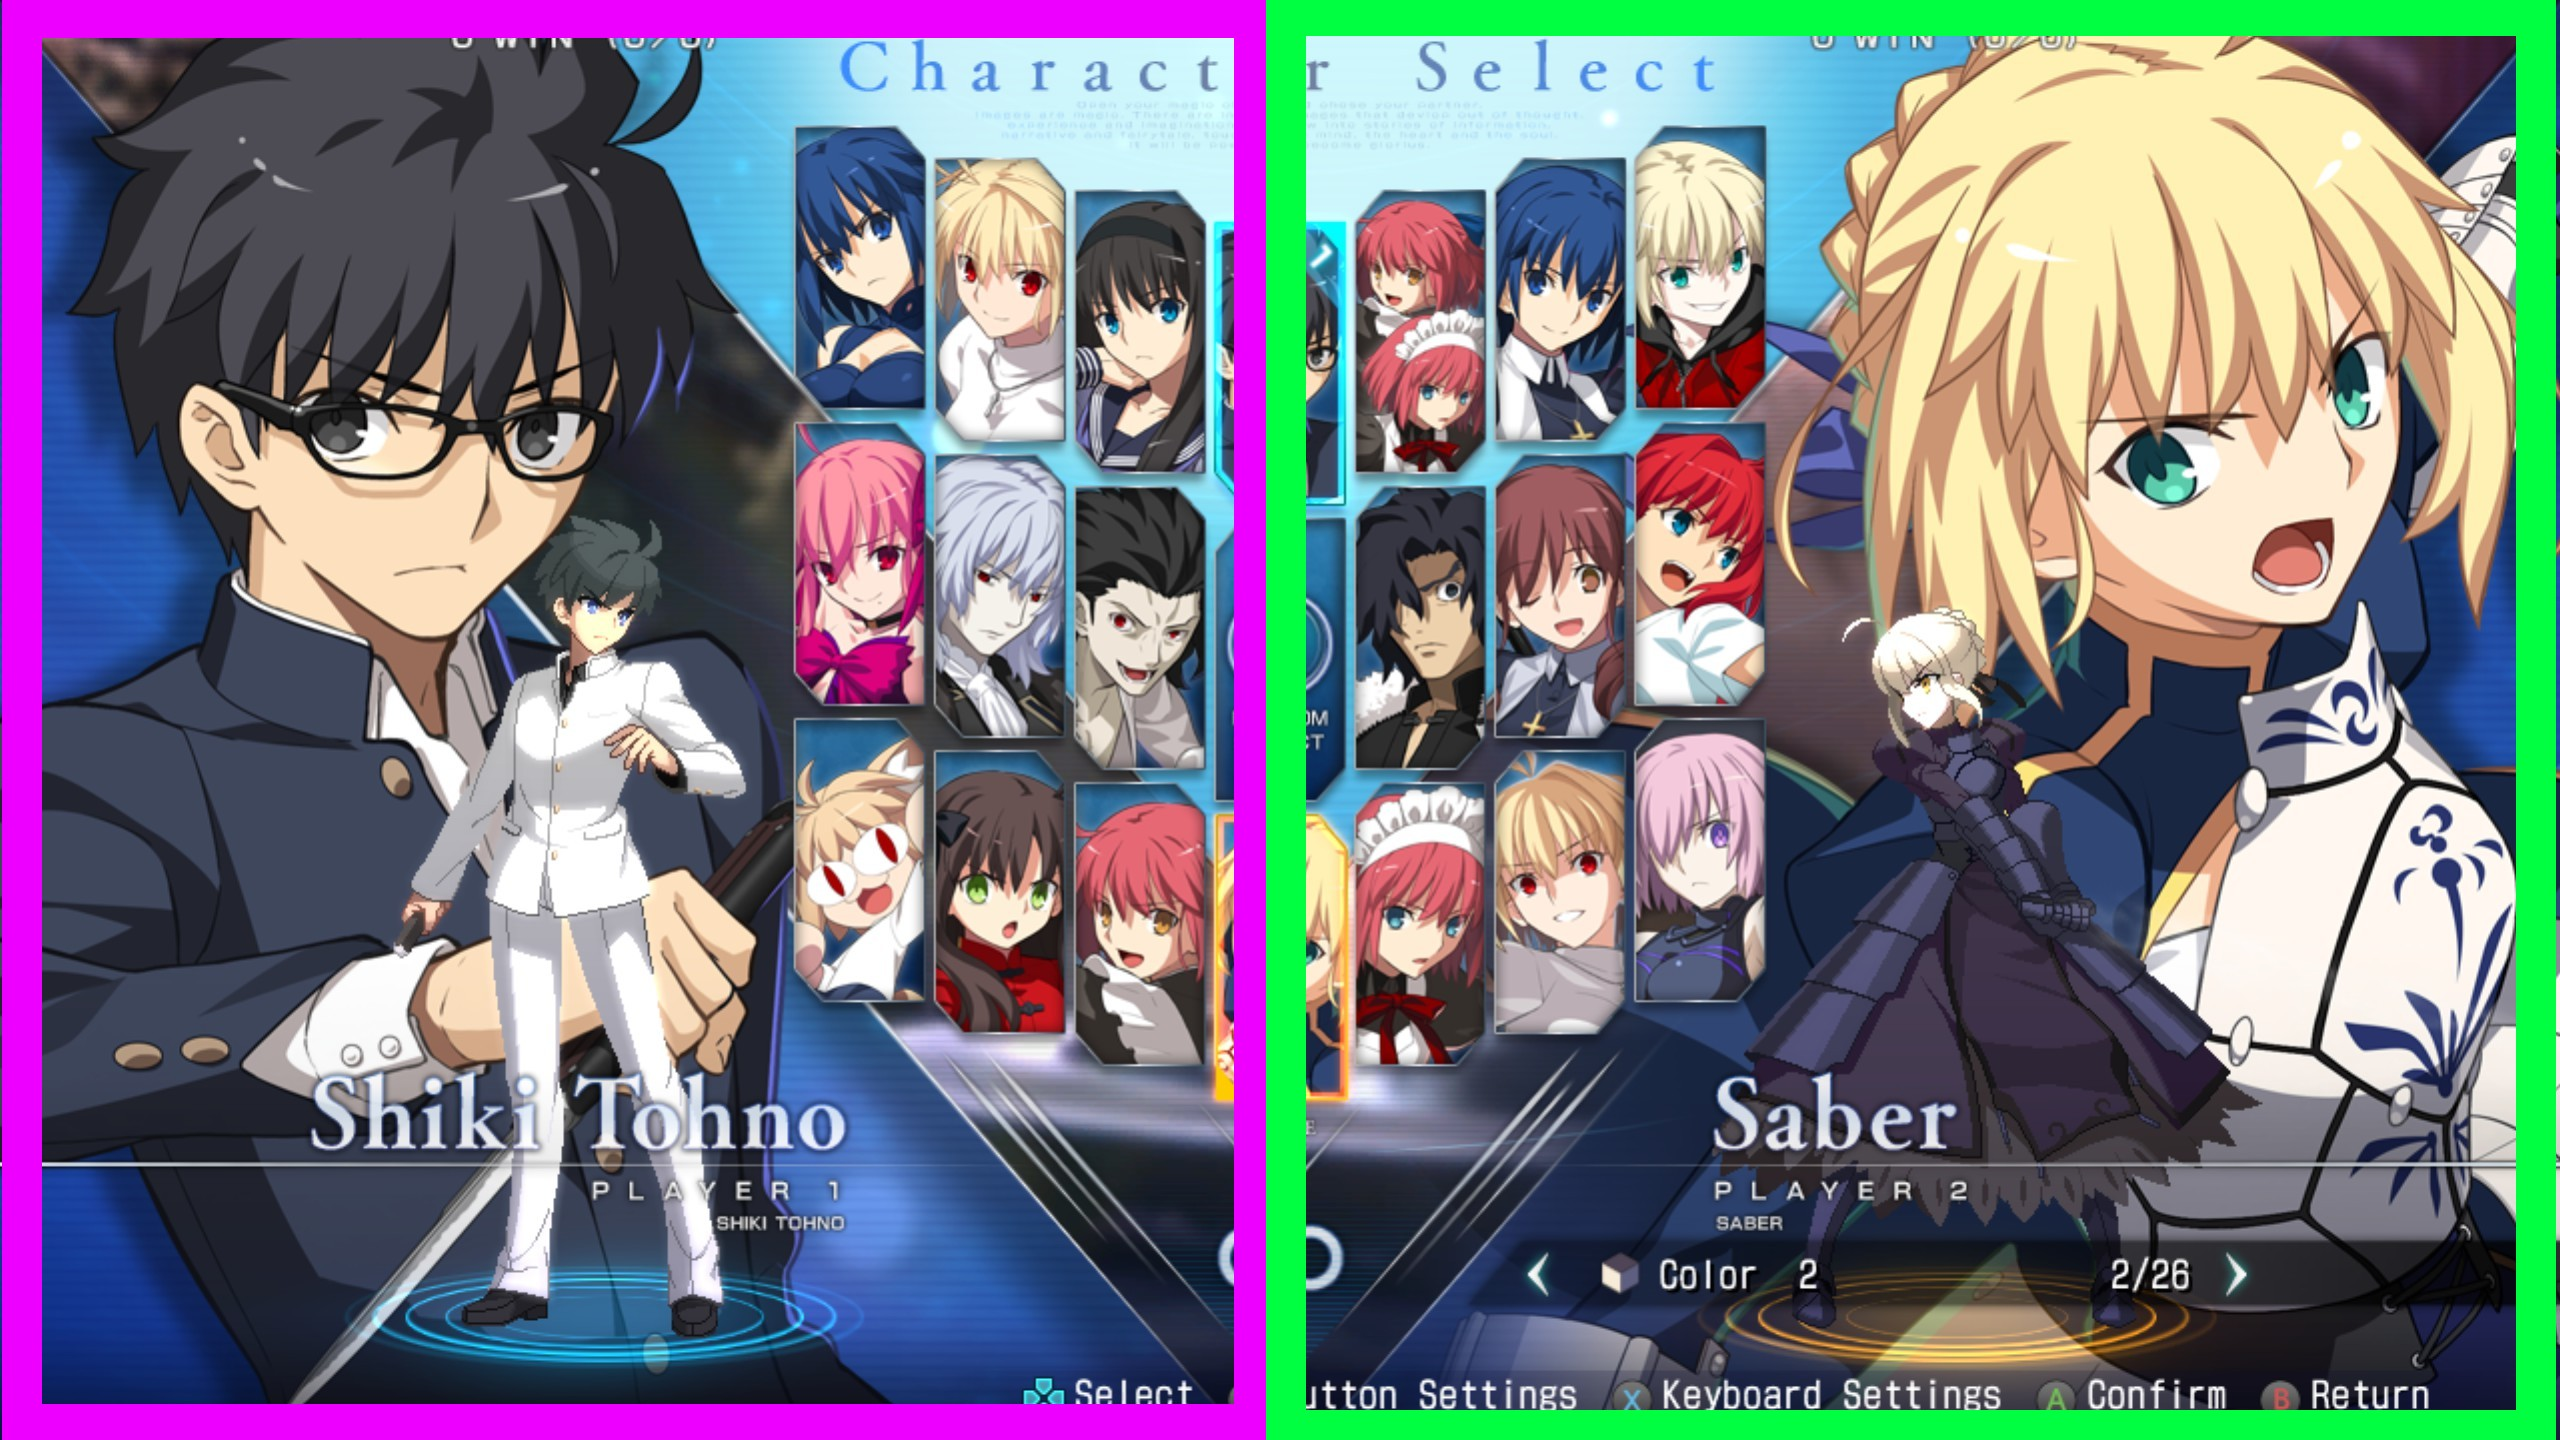
\includegraphics[height=0.5\textwidth]{figures/melty.jpg}
    \label{fig: melty character select}
\end{figure*}

Como se ve en ambos ejemplos, los personajes seleccionados están colocados en esquinas opuestas, cada uno en su propia caja. El único elemento que se comparte entre los dos es la lista de personajes

\textbf{Características de la interfaz gráfica}: 

\begin{itemize}
    \item Aspectos ergonómicos
    \item Colores
    \item Interactividad
    \item Validación de datos
    \item Consistencia
    \item Carga de memoria
    \item Indicaciones visuales
\end{itemize}